\documentclass[11pt, a4paper]{article}
\usepackage{multicol}
\usepackage{listings}
\usepackage{amsmath}          
\usepackage{amssymb}
\usepackage{graphicx}
\usepackage{subfig}
\usepackage{mathtools}
\usepackage{xcolor}
\usepackage{url}
\usepackage{fancyhdr}
\usepackage[T1]{fontenc}
\usepackage[utf8]{inputenc}
\usepackage[french]{babel}
\usepackage[left=2.5cm,right=2.5cm,top=2cm,bottom=3.5cm]{geometry}
\usepackage{xcolor}
\definecolor{codegreen}{rgb}{0,0.6,0}
\definecolor{codegray}{rgb}{0.5,0.5,0.5}
\definecolor{codepurple}{rgb}{0.58,0,0.82}
\definecolor{backcolour}{rgb}{0.95,0.95,0.92}

\colorlet{darkGreen}{green!30!black!70!}

\lstdefinestyle{mystyle}{
    language=C,
    backgroundcolor=\color{backcolour},   
    commentstyle=\color{codegreen},
    keywordstyle=\color{magenta},
    numberstyle=\tiny\color{black},
    stringstyle=\color{codepurple},
    basicstyle=\ttfamily\footnotesize,
    breakatwhitespace=false,         
    breaklines=true,                 
    captionpos=b,                    
    keepspaces=true,                 
    numbers=left,                    
    numbersep=5pt,                  
    showspaces=false,                
    showstringspaces=false,
    showtabs=false,                  
    tabsize=2
}

\lstset{style=mystyle}

\begin{document}

%----------- Informations du rapport ---------

\title{Projet Sandwich} %Titre du fichier .pdf
\newcommand{\sujet}[1]{Rapport de projet S5} %Nom du sujet
\newcommand{\enseignant}[1]{M. Jean-luc \textsc{BIENVENU}} %Nom de l'enseignant

\newcommand{\eleves}{Asia \textsc{AUVILLE}\\
Brice \textsc{TAGO}} %Nom des élèves

%----------- Initialisation -------------------
\begin{center}

\includegraphics[scale=0.3]{logo.png}~\\[2cm]
\end{center}
\begin{center}
    \textsc{\Large Rapport de projet S5}\\[1.5cm]
\end{center}
    % Title
     \rule{\linewidth}{0.2 mm} \\[0.6 cm]
     \begin{center}
	{\huge\bfseries Projet Sandwich}\\[0.6cm]
        \end{center}
    \rule{\linewidth}{0.2 mm} \\[1.5 cm]
	\vspace{1cm}%Espace de 3cm

    % Author and supervisor
    \begin{minipage}{0.4\textwidth}
      \begin{flushleft} \large
        \textbf{réalisé par : }\\
        Asia \textsc{AUVILLE}\\
        Brice \textsc{TAGO}
      \end{flushleft}
    \end{minipage}
    \begin{minipage}{0.4\textwidth}
      \begin{flushright} \large
        \textbf{Encadrant :}\\
         M. Jean-Luc \textsc{BIENVENU}\\
        
      \end{flushright}
    \end{minipage}

    \vfill

    % Bottom of the page
\begin{center}
    {\large 7 janvier 2022}
\end{center}
\newpage
\begin{center}
\tableofcontents
\end{center}
\newpage
\pagestyle{fancy}
\fancyheadoffset{1cm}
\setlength{\headheight}{2cm}
\lhead{
\includegraphics[scale=0.1]{logo.png}} %Affichage de l'image au top de la page
\rhead{\nouppercase{\leftmark}}
\rfoot{\thepage}
\cfoot{Rapport de projet S5}
\lfoot{}

\section{Introduction}

Dans ce rapport nous allons présenter notre travail effectué lors des derniers mois sur le projet "Sandwich", traitant des automates cellulaires et notamment du jeu de la vie. Nous aborderons point par point les grandes structures générales utilisées dans notre code, et leur évolution au cours des séances de projet. Les grandes parties qui seront traitées sont le fonctionnement du monde, des règles, de la file, des conflits, des options, de l'algorithme global ainsi que des tests effectués. 
\section{Présentation}

\subsection{Sujet}

Le sujet Sandwich est un sujet traitant d'automates cellulaires. Le but était de créer un univers et un ensemble de règles permettant de faire évoluer des cellules dans un espace donné. Ce système peut permettre d'implémenter par exemple le jeu de la vie de John Conway qui fait naître ou mourir des cellules dans un monde en deux dimensions selon des règles bien définies.
Dans ce projet, nous avons programmé une base permettant d'implémenter le jeu de la vie, puis au fil des achievements nous avons modifié et amélioré chaque structure pour augmenter l'efficacité et la praticité du code, ainsi que pour ajouter des fonctionnalités variées telle que le changement de couleur ou le déplacement des cellules.

\subsection{Cadre de travail}

Nous avons travaillé tous les deux en parallèle sur l'éditeur Emacs. Nous avons conçu le code ensemble dans sa globalité et nous avons favorisé le travail à deux sur une même tâche à la séparation des tâches, afin de confronter nos deux points de vue sur le code simultanément.  Néanmoins, c'est en particulier Brice qui s'est occupé de la gestion des conflits et des règles, et Asia qui s'est occupée de la file, de l'algorithme global de la fonction \textit{main}
\begin{figure}[!h]
    \centering
    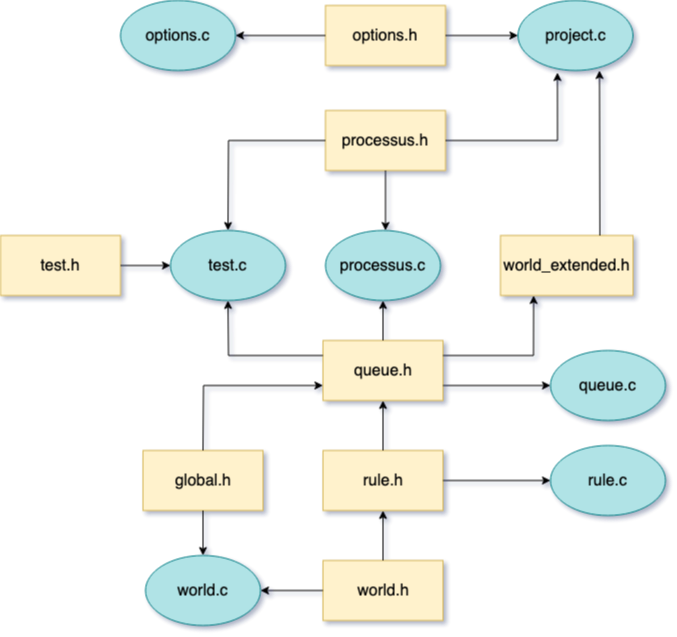
\includegraphics[scale=0.4]{diagramme.png}  
    \caption{Diagramme de dépendances}
    \label{}
\end{figure}

Ce graphique représente les dépendances des fichiers dans notre code, une flèche allant de A vers B signifie que que le fichier A est inclus dans le fichier B à l'aide d'un \#include .

\section{Corps du projet}

\subsection{Structure de monde}

Le monde est représenté par une structure contenant un tableau de taille WIDTH $\times$ HEIGHT, qui sont des constantes définies dans le makefile. Chaque case du tableau représente une cellule du monde et contient l'entier représentant sa couleur. Le tableau est organisé de telle sorte que la première case corresponde à la cellule la plus en haut à gauche du tableau, puis les cases sont réparties ligne par ligne de haut en bas. 

Nous avons alors une fonction indexes qui à partir des coordonnées i et j d'une cellule dans la matrice renvoie l'indice de la case correspondante dans le tableau contenu dans la structure de monde. 

Pour la création d'un jeu de la vie, nous avons créé un algorithme qui parcourt le tableau de la structure world et qui à chaque case génère un nombre aléatoire qui déterminera si la case sera blanche ou noire:

\begin{lstlisting}[frame= single]
    struct world create_game_of_life()
    {
        struct world game_of_life;
        for( int i =0; i<(WIDTH * HEIGHT); ++i){
        game_of_life.t[i] = WHITE * (rand()%2);
        }
        return game_of_life;
    }
\end{lstlisting}


Cet algorithme a une complexité linéaire par rapport au nombre de cellules, comme la plupart des programmes qui s'appliquent au monde, ce qui est raisonnable et efficace pour notre code. Nous avons également d'autres algorithmes qui créent des mondes différents selon nos besoins, par exemple pour les tests. 


Pour modifier l'initialisation du monde, nous appelons la fonction dont nous avons besoin dans la fonction \textit{world\_init} et nous modifions le code à chaque fois. Nous avions l'idée de remplir un tableau avec des pointeurs vers ces différentes fonctions afin d'ajouter une option lors de l'exécution de notre code pour créer un monde sur mesure, mais cela n'a pas été réalisé par manque de temps.

Finalement, la structure de monde a subi très peu de changements car elle était déjà adaptée dès le début. La fonction qui a été modifiée le plus est la fonction \textit{world\_apply\_rule}. Cette fonction au début ne prenait en compte que les règles de changement de couleur, elle modifiait alors la cellule du monde passée en argument en changeant l'entier contenu dans la case correspondante du tableau: il était alors remplacé par l'entier de la nouvelle couleur.
Cependant, lorsque nous avons implémenté les déplacements de case, cette manière de faire est devenue obsolète.
La nouvelle fonction fait donc deux actions au lieu d'une: premièrement, elle transforme la case concernée par le déplacement en une case noire. Ensuite, elle transforme la case d'arrivée du déplacement en la couleur définie par la règle:

\begin{lstlisting}[basicstyle=\footnotesize,frame = single][H]
void world_apply_rule(struct world* w, struct queue *queue, int indice)
{ 
    w->t[ (queue ->file[indice]).cases]= BLACK;
    w->t[ (queue -> file[indice]).arrival]= (queue -> file[indice]).couleur;
}
\end{lstlisting}


Cette manière de procéder fonctionne alors même lorsque la case concernée ne se déplace pas. En effet, la fonction va changer la couleur de la case en noir puis la changer à nouveau en la couleur définie. La première transformation est cependant inutile, et il aurait pu être judicieux de rajouter une condition pour ne pas l'appliquer si la cellule ne se déplace pas, afin d'améliorer la complexité de l'algorithme.

Pour afficher un monde nous avons la fonction \textit{world\_disp} qui affiche par ligne et colonne les nombres correspondant aux couleurs. Ci-dessous un exemple d'exécution du programme en taille 4x3 avec un seul monde affiché dans la sortie standard du terminal:
\begin{figure}[!h]
    \centering
    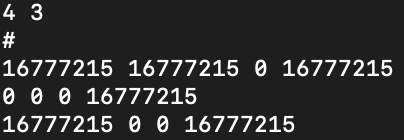
\includegraphics{world_disp.png}
    \caption{Monde en 4x3 généré aléatoirement}
    \label{fig:my_label}
\end{figure}

\subsection{Structure de règles}

Afin de reproduire le comportement évolutif des automates cellulaires, il nous a fallu implémenter des règles. 
Chaque règle est représentée par une structure dont les différents champs rendent comptent de notre cheminement mais aussi de notre conception de ce qu'est une règle.
\\

En effet pour nous, une règle correspond à un état particulier d'une cellule et de ses voisines et des transformations introduites par cet état. Il fallait donc que notre structure rule rend compte de tous ces aspects. 
Ainsi elle doit permettre de stocker la couleur de la cellule à laquelle la règle est censée s'appliquer, de stocker l'état de ses voisines, de stocker les différentes transformations possible c'est-à-dire les différentes couleurs que permettent la règle et les déplacements associés    


Chaque règle contient donc dans cet ordre:
\begin{itemize}
    \item La couleur de la cellule à laquelle elle s'applique qui est un entier contenu dans le champ \textit{center\_color}.
    \item Un booléen \textit{} qui permet de caractériser la règle c'est-à-dire si celle-ci requiert un motif particulier ou non.
    \item Un tableau d'entier qui selon que la règle est à motif fixe ou non, sert soit à stocker les différentes couleurs qu'utilise la règle ou à représenter sous forme de tableau le motif.
    \item Un tableau d'entier \textit{color\_iteration} qui dans le cas d'une règle à motif non fixe contient le nombre d'occurrence de chaque couleur nécessaire à l'application de la règle.
    \item Un entier pour le nombre de couleurs.
    \item Un tableau contenant les différents changements possible, c'est-à-dire les différentes couleurs que pourraient prendre la cellule affectée par la règle.
    \item Un tableau pour les différents déplacement qu'introduit la règle 
    \item Un entier donnant le nombre de changement permis par la règle. 
    
\end{itemize} 

Le choix d'une telle implémentation des règles est motivé par le fait que ce soit la méthode qui pour nous était la plus facile à mettre en oeuvre.
Les règles sont stockées dans un tableau qui se trouve dans le fichier \textbf{rule.c}, auquel nous n'avons pas accès depuis des fonctions extérieures. Alors, la manipulation de la structure rule se fait grâce à différentes fonctions implémentées dans ce fichier qui vont faire l'intermédiaire entre ce tableau et les autres fonctions de tout le code. Leur complexité reste très raisonnable, souvent en temps constant (linéaire pour la plus complexe). Certaines de ces fonctions permettent des manipulations basiques des règles, notamment pour pouvoir connaître le nombre de règles \textit{rules\_count}, pouvoir choisir une règle \textit{rule\_get}, pouvoir accéder au différents champs des règles et à leurs éléments \textit{rul\_num\_change}, \textit{rule\_change\_to}, \textit{rule\_change\_dx}, \textit{rule\_change\_dy}. D'autres permettent une manipulation plus avancée des règles à l'instar de la fonction \textit{ rules\_init },  qui permet de donner vie aux différentes règles en les initialisant et en les stockant dans le tableau évoqué plus haut, et de la fonction \textit{rule\_match} qui, elle, permet de vérifier la correspondance entre une règle et une cellule pour pouvoir par la suite appliquer les transformations qui s'imposent en cas de correspondance.


Cette fonction est non seulement longue et compliquée à lire et comprendre du point de vue d'un programmeur, mais elle est également trop générale pour des règles qui pourraient être vérifiées en deux lignes. L'algorithme consiste à vérifier si la règle concerne un pattern fixe et dans ce cas là vérifier si le voisinage de la case concernée correspond aux conditions, et si la règle se base sur un certain nombre de voisins de couleurs données alors il faut vérifier qu'il y a bien correspondance. 
Cette fonction est alors en même temps trop générale pour des règles simples mais également elle ne permet d'implémenter que des règles avec des conditions fixes. Sa complexité est cependant en temps constant donc elle est efficace au niveau temporel. 


Outre les problèmes liés à la conception des différentes fonctions, \textit{rule\_match} notamment et de la structure rule qui se doit d'être la plus générale possible c'est-à-dire s'adapter à tout type de règle, l'autre grande problématique était l'initialisation des règles. En effet nos choix de conception nous imposent pour chaque règle d'initialiser chaque champ en dur. Bien que cette manière soit possible, elle peut vite alourdir le code. 


Aussi, à partir de l'achievement 4, la structure rule change du tout au tout. les règles sont désormais construites à partir de \textit{Pointeurs de fonctions} qui s'adaptent mieux au caractère générique des règles. Désormais pour initialiser une règle, il faut implémenter une fonction qui vérifie si les cellules du monde valident la règle, et qui retourne un booléen qui permettra de savoir si la règle s'applique ou pas. La nouvelle structure rule est la suivante:\\

\begin{lstlisting}[frame = single]
struct rule
{
  int (*match)(const struct world*, unsigned int, unsigned int); //pointeur  
  int new_center_color[MAX_CHANGES]; //couleurs possibles apres transformations          
  struct couple deplacement[MAX_CHANGES]; //deplacements possibles    
  int nb_of_changes; //nombre de transformations differentes possibles
};
\end{lstlisting}

Elle conserve certains champs qui concernent les modifications apportées par la règle en cas de match avec une cellule donnée (c'est à dire les changements de couleur, les déplacements associés, et le nombre de modifications possible) 

Avec le changement de la structure rule, des modifications ont été apportées sur les fonctions \textit{rule\_match} et \textit{rules\_init}. Ci-dessous en guise d'exemple la nouvelle fonction d'initialisation des règles du jeu de la vie, beaucoup plus légère:\\

\begin{lstlisting}[frame = single][H]
    void rules_init_game_of_life()
        {
            struct rule rule1; struct rule rule2;
            rule1.match = &match_rule1_gol;
            rule2.match = &match_rule2_gol;
            rule1.new_center_color[0]= WHITE;
            ...
            rules[0] = rule1;
            rules[1] = rule2;
            NB_RULES = 2;
        }
\end{lstlisting}
On passe d'une fonction d'initialisation comprenant une dizaine de règles et faisant presque 100 lignes à une fonction considérablement plus courte et claire. On gagne également considérablement en complexité spatiale en choisissant de stocker des pointeurs de fonction et non de multiples tableaux inutiles. En choisissant d'implémenter les règles selon les conditions d'application directement on gagne en temps et en lisibilité. Nous avons simplement dû ajouter deux fonctions jouant le rôle de la fonction désormais obsolète \textit{rule\_match}, qui vérifient si il y a correspondance entre la règle donnée et la cellule, et les pointeurs de ces fonctions sont alors enregistrés dans la structure rule.

Nous pouvons avoir une vision concrète du monde généré. Voici un exemple de monde généré en taille 10x10 avec les règles du jeu de la vie et un monde \"planeur\", cas particulier et bien connu du jeu de la vie, à deux étapes successives d'affichage:

\begin{figure}[!h]
    \subfloat[planeur état 1]{
        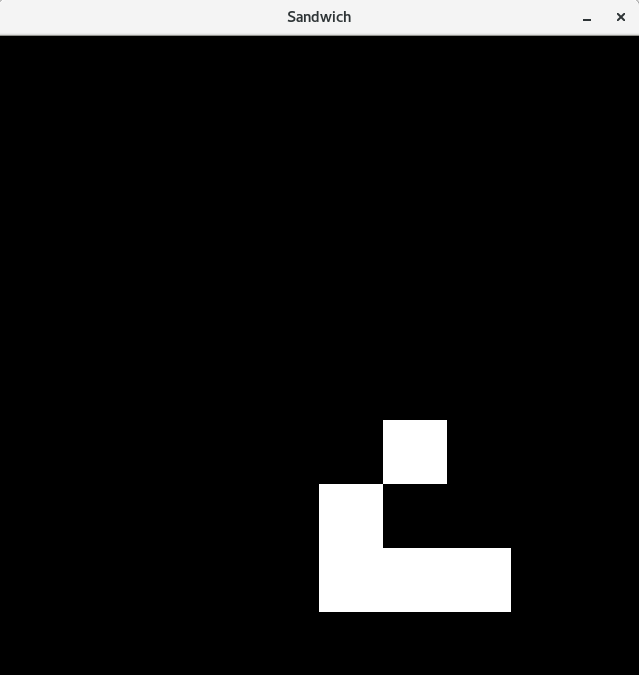
\includegraphics[scale = 0.2]{world1.png}
    }
    \hfill
    \subfloat[planeur état 2]{
        
\includegraphics[scale = 0.2]{world2.png}
    }
\end{figure}


\subsection{Structure de file}

Une fois que le lien entre une case et une règle est établi, il nous fallait pouvoir stocker cette case et les changements qui lui seront opérés. C'est la file qui sert d'endroit de stockage aux différents changements d'état des cellules.
La file est représentée par une structure contenant un tableau de struct cell et de deux entiers nous permettant de nous repérer dans le tableau: \textit{indice\_debut} qui correspond à l'indice du sommet de la file et \textit{indice\_fin} qui correspond à l'indice dans le tableau de la première case vide à la fin de la file, juste après son dernier élément:

\begin{lstlisting}[frame = single]
    struct queue
    {
        int indice_debut; //marque le debut de la file
        int indice_fin;  //marque la fin de la file
        struct cell file[WIDTH * HEIGHT * MAX_RULES] //elements de la file
    };
\end{lstlisting}
Une \textit{cell} dans le contexte de notre file est une structure contenant la couleur du changement qui doit être effectuée sur la case,
l'indice dans le monde de cette case, la case sur laquelle celle-ci est censée arriver si jamais la règle avec laquelle elle match introduit un déplacement (et elle même dans le cas échéant, c'est le déplacement "nul") et un booléen nous permettant de décider si oui ou non la règle est "activée", c'est à dire est-ce qu'elle sera prise en compte lors de l'application des règles (utile pour la gestion de conflits).\\

\begin{lstlisting}[frame = single]
struct cell 
{
  int couleur; //nouvelle couleur apres transformation
  int cases; //cas d'application de la regle
  int arrival; //case d'arrivee
  int booleen; //etat d'activation de la regle
};                      
\end{lstlisting}

Un tel choix de conception de la file se justifie par un soucis d'optimisation tant au niveau de la lisibilité du code qu'au niveau de la complexité. En effet la première structure de file implémentée était conçue à partir de multiples tableaux qui représentaient chacun des champs de la structure cell en plus des deux entiers \textit{indice\_debut} et \textit{indice\_fin}. Cette méthode de conception bien que fonctionnelle impliquait de parcourir à chaque fois plusieurs tableaux pour avoir accès aux différentes informations. Par l'utilisation de la structure cell, on se restreint à un unique tableau \textit{file}, gagnant autant en espace qu'en temps d'exécution. Ce choix est aussi dû à notre maîtrise de la conception de tableaux par rapport au concept de liste chaînée qui fut envisagée puis abandonnée par la suite. \\
A l'instar de la structure rule, la manipulation de la structure file se fait à partir de fonctions. 

\noindent Ainsi nous avons : 
\begin{itemize}
    \item une fonction de création de file vide \textit{queue\_init}.
    \item  une fonction \textit{queue\_append} d'ajout d'éléments dans la file, dans laquelle pour chaque cellule on fait le choix aléatoire de la transformation qui lui sera appliquée (parmi celles permises par la règle).
    \item une fonction \textit{queue\_pop} de retrait du premier élément dans la file, qui agit en incrémentant indice\_debut.
\end{itemize}


\subsection{Gestion des conflits}

\label{GC}
Une des propriétés majeures des automates cellulaires est qu'ils permettent aux cellules de se déplacer. Ainsi pour se rapprocher au plus du comportement de ces automates, il nous a fallu introduire la notion de déplacement et ceci dès l'achievement 2. Cependant celle-ci soulève un problème: comment gérer plusieurs cellules qui auraient la même case d'arrivée, ou une cellule qui voudrait se déplacer sur une case déjà occupée ? On parle de conflit.\\


Il nous a donc fallu mettre en place des méthodes de gestions des conflits qui n'impliqueraient pas de sacrifier des particules. \\

S'il fût dans un premier temps décidé qu'en cas de conflit la priorité serait donnée à la dernière particule dans l'ordre de la file, cette méthode sera vite abandonnée au profit d'une autre qui permet de conserver toutes les cellules. Elle consiste à choisir aléatoirement une cellule parmi toutes celles qui prétendent à une même case. Concrètement, il s'agit pour nous de parcourir notre file, et pour chaque case d'arrivée potentielle induite par une transformation, vérifier si il y a un conflit. Dans ce cas, on choisit aléatoirement une transformation parmi les prétendantes puis on la garde en dépit des autres. \\

La plus grande difficulté était alors de "désactiver" les autres transformations. Si une méthode envisagée fut de les supprimer, nous avons finalement opté pour une méthode qui utilise un booléen. Ce booléen va servir à marquer la struct cell. En effet une transformation dont le booléen est à 0 sera considérée comme désactivée et ne s'appliquera donc pas à la case prévue. Au départ, tous les booléens sont initialisés à 0, et lorsqu'une transformation est choisie aléatoirement ou ne fait l'objet d'aucun conflit, la valeur de son booléen devient 1. Cette manière de procéder nous a permis d'outrepasser un des problèmes que posait l'utilisation de tableau pour la conception de notre file, à savoir comment supprimer un élément de notre choix dans un tableau sans devoir en faire une copie, ce qui aurait augmenté considérablement la complexité de notre algorithme.

La complexité temporelle actuelle de notre algorithme de gestion des conflits est quadratique, car il contient une boucle générale parcourant la file puis plusieurs sous boucles s'exécutant dans celle ci et parcourant la file ou un tableau de taille similaire à chaque fois. A notre échelle, l'exécution est très fluide et nous ne remarquons aucune latence. Cependant, avec un plus grand nombre de cases et de règles, il est possible que la complexité temporelle pose problème au bon fonctionnement du code.

\subsection{Options}

En plus des spécifications sur les données écrites sur la sortie standard notamment celle sur l'affichage qui définit comment devaient être représentées les données de sorties à l'écran et celle sur la possibilité de changer la taille de l'image définie dans le Makefile, il était demandé  de pouvoir choisir le nombre d'images produites au travers de l'option \textit{-m} et de pouvoir fixer le déroulement des évènements par initialisation du générateur aléatoire c'est-à-dire fixer la suite des images produites grâce à l'option \textit{-s}. 

La mise en place de ces différentes options se fait au moyen de la fonction \textit{getopt} de la bibliothèque du même nom appelée dans la fonction \text{remplir\_struct}. Le but ici est d'analyser les données de la ligne de commande accessible grâce aux paramètres \textit{argc} et \textit{argv} de la fonction \textit{main}. Les différentes sorties obtenues servent à initialiser les champs d'une structure \textit{opt}.
En ayant accès à ces champs, on récupère ainsi les valeurs définies par l'utilisateur pour les différentes options \textit{\-m} et \textit{\-s} grâce aux fonctions \text{get\_s} et \textit{get\_m} qu'on utilisera ensuite respectivement pour la boucle \textit{for} principale qui donne le nombre d'image et pour l'initialisation du générateur aléatoire \textit{rand}

 Ces options sont un excellent moyen de se rendre compte d'un quelconque dysfonctionnement de notre code même s'ils restent insuffisants pour décider de la correction de celui-ci.
Avoir le contrôle sur le nombre d'images produites nous permet de choisir un nombre suffisant de "frames" (donc d'itérations de la boucle de la fonction main) et connaître comment devrait se dérouler les évènements nous permet de repérer le problème.

Une amélioration possible pour notre code aurait été d'implémenter un système d'options permettant de choisir quel monde et quelles règles nous voulons initier lors de la compilation.

\subsection{Algorithme global de la fonction main}
Explication de l'ordre des appels des fonctions et de comment tout notre code se lie grâce à cet algorithme global.

Pour lier toutes ces structures, nous avons deux fichiers .c principaux: \textbf{processus.c} et \textbf{project.c}.
\textbf{project.c} est le fichier contenant la fonction \textit{main}, c'est celui qu'on exécute lorsque l'on veut faire fonctionner le programme. 
Il s'articule selon plusieurs étapes nécessaires et obligatoires au fonctionnement du code. 

Le sujet donnait comme instruction de base l'algorithme suivant:

\begin{figure}[!h]
    \centering
    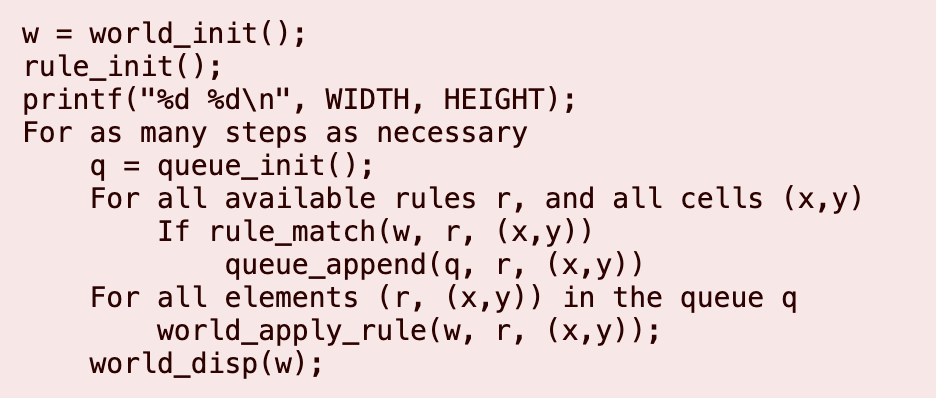
\includegraphics[scale=0.7]{./algo_sujet.png}
    \caption{algorithme du main() prévu dans le sujet}
    \label{fig:my_label}
\end{figure}

Nous avons alors en premier lieu implémenté une fonction qui reproduit exactement l'algorithme demandé, car il était assez adapté à l'achievement 0 et aux premières étapes de notre réflexion. 
Cet algorithme fonctionne de la manière suivante: 
\begin{itemize}
    \item En premier lieu, on initialise un monde selon les règles définies (voir la section dédiée aux mondes).
    \item On initialise ensuite les règles de la même manière.
    \item On affiche dans la sortie standard les dimensions du monde généré afin qu'il puisse être affiché correctement par l'interface graphique sdl fournie dans le sujet.
    \item On rentre dans la première boucle: celle-ci correspond à une itération de modifications sur le monde, donc une image affichée par l'interface graphique
    \item On initialise la file qui contiendra l'ensemble des règles à appliquer aux cellules du tableau: elle est sûrement déjà remplie d'autres instructions correspondant aux tours d'avant donc il faut la réinitialiser.
    \item Puis on itère sur chaque case et sur chaque règle pour tester quelle case vérifie les conditions des règles, si c'est le cas on ajoute la règle et la case correspondante au bout de la file.
    \item On parcourt alors la file depuis le début et on applique chaque modification enregistrée aux cellules du tableau. Les modifications ne sont pas faites directement et doivent être stockées dans une file car sinon elles changeraient les conditions de vérification des règles des cases voisines et fausseraient l'algorithme.
    \item Enfin, on affiche le monde dans la sortie standard avec les modifications effectuées. Cet affichage se fait dans la boucle des modifications sur le monde, c'est à dire qu'il se fait autant de fois que l'on demande de modifications et de "captures" du monde différentes.\\
    
\end{itemize}
Cependant, au fur et à mesure de l'avancement dans le projet, nous avons été confrontés à des problèmes avec cet algorithme, notamment lorsque nous avons modifié la structure de file et les règles, et que nous avons rajouté le système de gestion de conflits. Nous ne pouvions plus nous permettre de juste appliquer les règles après les avoir stockées dans la file car il fallait appliquer nos procédures de gestion des conflits afin de pouvoir activer les règles choisies. \\
Par conséquent, nous avons dû modifier le programme et créer une deuxième version:

\begin{lstlisting}[frame= single][H]
    int main( int argc, char * argv[])
        {
            struct options opt; 
            remplir_struct( &opt, argc, argv); //definition des options
            srand( get_s(&opt);
            struct world w = world_init(); //initialisation du monde
            rules_init(); //initialisation des regles
            printf("%d %\n", WIDTH, HEIGHT);
            struct queue queue;
            world_disp(&w); //affichage du monde avant transformation
            for( int i=0; i<get_m(opt); ++i){
                struct queue *q =queue_init(&queue);
                queue_fill(q,&w);
                gestion_conflits(q,&w);
                application_regles(q,&w);
                world_disp(&w);
            }
        }
\end{lstlisting}

Le début de la fonction est similaire. Nous avons ajouté les fonctionnalités des options lors de l'exécution du code donc nous devons les initialiser, et nous choisissons d'afficher le monde une fois avant les premières modifications. 
\\ Par la suite, nous avons décidé de séparer les instructions qui s'appliquent à chaque appel de la boucle \textbf{for} en 3 parties. Ces fonctions sont écrites dans le fichier processus.c et sont construites de la manière suivante:
\begin{itemize}
    \item La première est la fonction \textit{queue\_fill}, qui va appeler plusieurs fonctions (déjà introduites précédemment) dans le but de vérifier quelle règle s'applique à quelle case et de remplir la file en conséquent.
    \item La deuxième fonction \textit{gestion\_conflits} contient les instructions de gestion des conflits et va activer les règles que l'on va exécuter par la suite.
    \item La dernière fonction applique les règles alors activées, et actualise la file au fur et à mesure avec les fonctions définies dans ce but.\\
\end{itemize}
Après ces procédures, on va évidemment afficher le monde qui résulte des modifications apportées, et cela à chaque itération de la boucle. 

Cette séparation en trois blocs des principales fonctions du programme permet premièrement de rendre le code plus lisible et compréhensible et deuxièmement de tester les fonctions à part dans le fichier test.c. En effet, si nous ne les avions pas séparées il aurait été impossible d'appeler project.c depuis test.c car les deux comportent une fonction main() et cela aurait causé un conflit. 

\subsection{Tests}

En premier lieu, les tests que nous effectuions se limitaient à une observation visuelle des résultats avec des exécutions du programme dans des conditions particulières. Cependant, cette méthode implique que certaines erreurs dans le code peuvent nous passer devant les yeux sans que nous les remarquions. Nous avons alors conduit plusieurs tests plus importants dans le fichier \textbf{test.c}.

Les tests sont dans la fonction \textit{main} du fichier et ont été effectués grâce à la fonction \textit{assert}, qui provoque une erreur de segmentation lors de l'exécution du code si la condition n'est pas effectuée.

\begin{lstlisting}[frame = single][H]
    struct world w = create_planeur();
    rules_init_game_of_life();
    for( unsigned int regle = 0; regle< rules_count(); regle++){
        assert(rule_match(&w, rule_get(regle), 1, 2) == 0 );
    }
\end{lstlisting}

Ce test a pour but de vérifier un cas particulier d'application de la fonction \textit{rule\_match}. A ce moment de code, notre jeu de la vie fonctionnait déjà et nous avions vu que les règles s'appliquaient sur les cases qui vérifiaient les règles, alors nous voulions surtout vérifier un cas où aucune règle ne devait s'appliquer sur la case.

Nous avons alors généré un monde simple de "planeur" qui est un exemple bien connu de monde de départ du jeu de la vie, tirant son nom de sa ressemblance avec un planeur qui se déplace en ligne droite dans l'univers créé. Nous avons ensuite testé la fonction \textit{rule\_match} grâce à un \textbf{assert} avec toutes les règles du jeu de la vie sur une des cases de ce monde qui ne devait valider aucune des règles. Lors de l'exécution du fichier, tout se passe correctement sans erreur de segmentation, on peut donc en déduire la validation de notre test.

\begin{lstlisting}[frame = single][H]
    struct queue q1; struct queue q2;
    struct queue *queue1 = queue_init(&q1);
    struct queue *queue2 = queue_init(&q2);
    queue_append(queue1, rule_get(0),1,4);
    queue_append(queue1, rule_get(1),1,5)
    queue_append(queue1, rule_get(1),1,5)
    assert(queue1 ->file[queue1->indice_debut].cases == 
                queue2 ->file[queue1->indice_debut].cases);
    assert(queue1 ->file[queue1->indice_fin].cases ==
                queue2 ->file[queue1->indice_fin].cases);
\end{lstlisting}

Ce test a pour but de vérifier la validité de nos primitives agissant sur notre structure de file d'attente. Nous avons créé deux files différentes, dans les quelles nous avons ajouté des transformations, de telle sorte à ce que l'unique transformation de la deuxième file soit en deuxième position de la première file. Ainsi, nous appliquons par la suite la fonction \textit{queue\_pop} à la première file et testons si les éléments en première position sont les mêmes. Lors de l'exécution tout se passe bien, le test est donc validé.

\begin{lstlisting}[frame = single][H]
struct world w1 = create_world_test_conflit();
int cases_vivantes_debut=test_incompressibilite(&w1,WIDTH*HEIGHT);
rules_test_incompressibilite();
struct queue queue;
for(int i=0; i<500; ++i){
    struct queue *q = queue_init(&queue);
    queue_fill(q, &w1);
    gestion_conflits(q,&w1);
    application_regle(q,&w1);
}
int cases_vivantes_fin = test_incompressiblite(&w1,WIDTH*HEIGHT);
assert(cases_vivantes_debut == cases_vivantes_fin);
return 0;
\end{lstlisting}

Ce test a été le plus important à mettre en place pour nous. Pour tester l'incompressibilité et la gestion de conflits, nous avons implémenté un système de règles qui ne supprime ni ne crée aucune case blanche et qui n'induit que des déplacements. Pour valider le système de gestion de conflits, nous avons donc voulu faire tourner l'algorithme un grand nombre de fois (en l'occurrence 500)  et comparer le nombre de cases blanches à la fin et au début à l'aide d'un \textbf{assert}. Si le système fonctionne, ces nombres seront égaux.


Pour pouvoir exécuter ce test, nous avons été contraints de séparer la fonction \textit{main} en plusieurs fonctions que nous avons déplacées dans \textbf{processus.c} afin de pouvoir y accéder depuis \textbf{test.c} sans devoir faire un copié collé du code. Cela a également permis de rendre le code plus lisible et compréhensible.\\

Ce test n'a pas été concluant immédiatement, et il nous a permis de déceler des erreurs dans notre code: Le programme calculant les voisins d'une case comportait une erreur liée au caractère torique du monde, les bordures causant alors des disparitions de cellules. Nous avons remarqué également grâce à ces tests que nous avions oublié d'activer (voir \ref{GC} ) les règles dans un certain cas, nous avons donc pu corriger l'erreur. Finalement, le test a été validé et a validé par la même occasion notre algorithme de gestion des conflits.
\section{Conclusion}

Ce projet nous a donc permis d'implémenter un système permettant de générer un espace cellulaire en deux dimensions et de faire évoluer des cellules en son sein à l'aide des règles définies. Il nous a également permis de mieux comprendre la compilation séparée, et nous avons acquis une meilleure maîtrise de la manipulation des fichiers \textbf{.h}. 

\end{document}

